% This is "sig-alternate.tex" V2.1 April 2013
% This file should be compiled with V2.5 of "sig-alternate.cls" May 2012
%
% This example file demonstrates the use of the 'sig-alternate.cls'
% V2.5 LaTeX2e document class file. It is for those submitting
% articles to ACM Conference Proceedings WHO DO NOT WISH TO
% STRICTLY ADHERE TO THE SIGS (PUBS-BOARD-ENDORSED) STYLE.
% The 'sig-alternate.cls' file will produce a similar-looking,
% albeit, 'tighter' paper resulting in, invariably, fewer pages.
%
% ----------------------------------------------------------------------------------------------------------------
% This .tex file (and associated .cls V2.5) produces:
%       1) The Permission Statement
%       2) The Conference (location) Info information
%       3) The Copyright Line with ACM data
%       4) NO page numbers
%
% as against the acm_proc_article-sp.cls file which
% DOES NOT produce 1) thru' 3) above.
%
% Using 'sig-alternate.cls' you have control, however, from within
% the source .tex file, over both the CopyrightYear
% (defaulted to 200X) and the ACM Copyright Data
% (defaulted to X-XXXXX-XX-X/XX/XX).
% e.g.
% \CopyrightYear{2007} will cause 2007 to appear in the copyright line.
% \crdata{0-12345-67-8/90/12} will cause 0-12345-67-8/90/12 to appear in the copyright line.
%
% ---------------------------------------------------------------------------------------------------------------
% This .tex source is an example which *does* use
% the .bib file (from which the .bbl file % is produced).
% REMEMBER HOWEVER: After having produced the .bbl file,
% and prior to final submission, you *NEED* to 'insert'
% your .bbl file into your source .tex file so as to provide
% ONE 'self-contained' source file.
%
% ================= IF YOU HAVE QUESTIONS =======================
% Questions regarding the SIGS styles, SIGS policies and
% procedures, Conferences etc. should be sent to
% Adrienne Griscti (griscti@acm.org)
%
% Technical questions _only_ to
% Gerald Murray (murray@hq.acm.org)
% ===============================================================
%
% For tracking purposes - this is V2.0 - May 2012

\documentclass{sig-alternate-05-2015}


\begin{document}

% Copyright
\setcopyright{acmcopyright}
%\setcopyright{acmlicensed}
%\setcopyright{rightsretained}
%\setcopyright{usgov}
%\setcopyright{usgovmixed}
%\setcopyright{cagov}
%\setcopyright{cagovmixed}


% DOI
% \doi{10.475/123_4}

% ISBN
% \isbn{123-4567-24-567/08/06}

%Conference
\conferenceinfo{MSR '16}{May 14--15, 2016. Austin, USA}

% \acmPrice{\$15.00}

%
% --- Author Metadata here ---
% \conferenceinfo{WOODSTOCK}{'97 El Paso, Texas USA}
%\CopyrightYear{2007} % Allows default copyright year (20XX) to be over-ridden - IF NEED BE.
%\crdata{0-12345-67-8/90/01}  % Allows default copyright data (0-89791-88-6/97/05) to be over-ridden - IF NEED BE.
% --- End of Author Metadata ---

\title{A Bug-Fix Metarepository for Developers and
Researchers}
%
% You need the command \numberofauthors to handle the 'placement
% and alignment' of the authors beneath the title.
%
% For aesthetic reasons, we recommend 'three authors at a time'
% i.e. three 'name/affiliation blocks' be placed beneath the title.
%
% NOTE: You are NOT restricted in how many 'rows' of
% "name/affiliations" may appear. We just ask that you restrict
% the number of 'columns' to three.
%
% Because of the available 'opening page real-estate'
% we ask you to refrain from putting more than six authors
% (two rows with three columns) beneath the article title.
% More than six makes the first-page appear very cluttered indeed.
%
% Use the \alignauthor commands to handle the names
% and affiliations for an 'aesthetic maximum' of six authors.
% Add names, affiliations, addresses for
% the seventh etc. author(s) as the argument for the
% \additionalauthors command.
% These 'additional authors' will be output/set for you
% without further effort on your part as the last section in
% the body of your article BEFORE References or any Appendices.

\numberofauthors{2} %  in this sample file, there are a *total*
% of EIGHT authors. SIX appear on the 'first-page' (for formatting
% reasons) and the remaining two appear in the \additionalauthors section.
%
\author{
% You can go ahead and credit any number of authors here,
% e.g. one 'row of three' or two rows (consisting of one row of three
% and a second row of one, two or three).
%
% The command \alignauthor (no curly braces needed) should
% precede each author name, affiliation/snail-mail address and
% e-mail address. Additionally, tag each line of
% affiliation/address with \affaddr, and tag the
% e-mail address with \email.
%
% 1st. author
\alignauthor
Mathieu Nayrolles\\
       \affaddr{Software Behaviour Analysis Research Lab}\\
       \affaddr{ECE, Concordia University,}\\
       \affaddr{Montr\'eal, Canada}\\
       \email{mathieu.nayrolles@concordia.ca}
% 2nd. author
\alignauthor
Abdelwahab Hamou-Lhadj\\
  \affaddr{Software Behaviour Analysis Research Lab}\\
  \affaddr{ECE, Concordia University,}\\
  \affaddr{Montr\'eal, Canada}\\
  \email{wahab.hamou-lhadj@concordia.ca}
}

\maketitle
\begin{abstract}
In recent years, mining bug report (BR) and their related fixes
has perhaps been one of the most active software
engineering research fields. There exists many open source and
many open source and
proprietary bug tracking and source code versioning systems
that developers and researchers can use to examine bug
reports so as to reason about software quality. The issue is
that these repositories use different interfaces and ways to
access and represent data, which hinders productivity and
reuse.
To address this, we introduce a large dataset of 700,000 fixed
bugs belonging to 1,900 different project. This dataset follows a
clear infrastructure and allows developers and researchers interested in
mining data from different (and heterogeneous) repositories to do so easily.
\end{abstract}


\keywords{Bug tracking systems; Source code versioning
systems; Bug Reports; Mining software repositories}

\begin{CCSXML}
<ccs2012>
<concept>
<concept_id>10011007.10011006.10011072</concept_id>
<concept_desc>Software and its engineering~Software libraries and repositories</concept_desc>
<concept_significance>300</concept_significance>
</concept>
</ccs2012>
\end{CCSXML}

\ccsdesc[300]{Software and its engineering~Software libraries and repositories}

\printccsdesc

% We no longer use \terms command
%\terms{Theory}


\section{Introduction}
\label{sec:Introduction}

Bug tracking systems such as Bugzilla and Jira have
grown to contain hundreds of thousands of bugs, providing
a vast amount of data to several active research fields
including bug reproduction, bug triaging, and empirical
studies. The analysis of BRs can provide useful insight that
can help with many maintenance tasks such as bug fixing
\cite{Weiß2007, Bhattacharya2011, Saha2014}, bug reproduction \cite{Artzi2008,Chen2013,Jin2012,Nayrolles2015}, bug prediction \cite{DAmbros2010, Kamei2010, Kim2011a}, and fault analysis \cite{Hamill2014}.

Today, there exist many bug tracking and source code
versioning tools (e.g., Bugzilla, Jira, SVN, Git, etc.) that
can be used by practitioners and researchers to conduct
large-scale studies on the causes and distribution of bugs in
software systems. The problem is that these systems have
different interfaces to access data. The data is not
represented in a uniform way either. This is further
complicated by the fact that bug tracking tools and code
versioning systems are not necessarily connected. The
former follows the life of the bug itself and not its fixes,
which are managed by the latter.
Analyzing the bugs and their fixes from different
sources require going back and forth between diverse tools,
creating parsers, mapping data from a repository to another,
etc. These tasks are not only time consuming but add no
value to the analysis itself.

For the time being, our dataset, which is available for download at
https://bumper-app.com/msr16, aggregates bug report and fixes from
Eclise\footnote{https://www.eclipse.org/}, Gnome\footnote{https://www.gnome.org/}, the Apache Software fundation\footnote{http://www.apache.org/} and Netbeans\footnote{https://netbeans.org/}.
Moreover, our dataset associates each bug report (bug description, reportee, assignee, comments, ...) and its related fixes.
These systems use Bugzilla\footnote{https://www.bugzilla.org/} or Jira\footnote{https://www.atlassian.com/software/jira} as their bug report system and Git\footnote{https://git-scm.com/} or Mercurial\footnote{https://www.mercurial-scm.org/} as their source code versioning engine.

\section{Data Collection}
\label{sec:Data Collection}

Figure \ref{fig:bumper-dc} illustrates how we extracted
data from various bug report tracking and code
versioning systems. In this example, we extract raw data
from two bug tracking systems, Bugzilla and Jira with their
corresponding source code versioning systems, Git and
Mercurial. The extracted data is consolidated in one
database where we associate
each bug report with its fix. Note that this association is
based on the general practice where developers create a link
between the bug tracking system and their source versioning
tool by either writing the bug \#ID in their commit message or
adding a link towards the changeset as a comment in the bug
report system. Algorithms for linking these two entities in
the absence of explicit linkage can also be used such as the
one presented by Wu et al. \cite{Wu2011} in their tool, Relink.


\begin{figure}
  \centering
  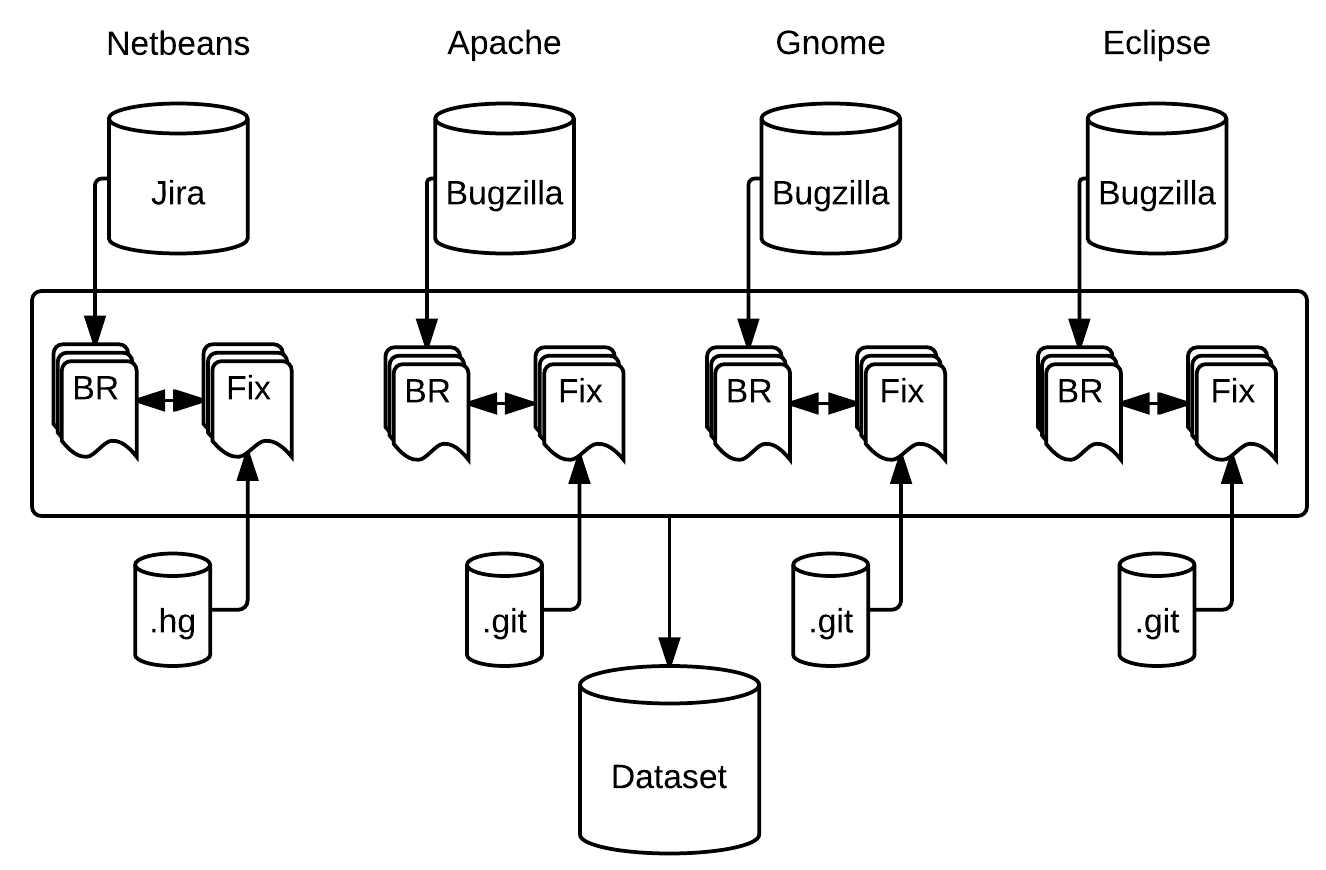
\includegraphics[width=0.45\textwidth]{media/dc.png}
  \caption{BUMPER Data Collection\label{fig:bumper-dc}}
\end{figure}


Currently, our dataset includes five bug report management systems, namely, Gnome, Eclipse, Netbeans and the Apache Software Foundation that are composed
of 512, 190, 39 and 349 projects respectively,
bringing the total of projects to 1,930.
These projects cover 16 years of development from 1999 to 2015.
Gnome is a free desktop environment, mainly developed in C and C++.
Eclipse and Netbeans are integrated development environments (IDEs) for
developing with many programming languages, including Java, PHP, and C/C++.
Finally, The Apache Software Foundation (ASF) is a non-profit public charity
established in 1999, that provides services and support for many like-minded
software project communities of individuals who choose to join the ASF.
The extracted data is consolidated in one database where we associate each bug report with its fix.
The fixes are mined from different types of version control systems.
Gnome, Eclipse and Apache Software Foundation projects are based on Git
 (or have git-based mirrors), whereas Netbeans uses Mercurial.
The characteristics of the five aggregated datasets
are presented in Table~\ref{tab:summary}.

We chose to use with these systems to have data coming from
diverse code versioning and bug tracking systems.
Also, Gnome, Eclipse, Netbeans and the Apache Software Foundation exhibit a
great deal of diversity in terms of the programming
languages used to build applications, development teams,
location of the development teams, utility, and maturity.
Moreover, they use different tools, Bugzilla, JIRA, Git, and
Mercurial. This said, we can and plan to integrate other datasets that
use any combination of these tools.

\begin{table}[]
\centering
\caption{
RESOLVED/FIXED BUG (R/F BR),  CHANGESETS (CS), AND
PROJECTS BY DATASET \label{tab:datasets}}
\label{tab:summary}
\begin{tabular}{c|c|c|c|c}
\textbf{Dataset} & \textbf{R/F BR} & \textbf{CS} & \textbf{Files} & \textbf{Projects} \\ \hline \hline
Gnome            & 550,869         & 1,231,354   & 367,245        & 512                \\ \hline
Netbeans         & 53,258          & 122,632     & 30,595         & 39                \\ \hline
Apache           & 49,449          & 106,366     & 38,111         & 349               \\ \hline
Eclipse          & 78,830          & 184,900     & 21,712         & 190                \\ \hline \hline
Total            & 732,406         & 1,645,252   & 457,663        & 1,930               \\ \hline \hline
\end{tabular}
\end{table}

As we can see from in Table \ref{tab:datasets}, our consolidated dataset contains 732,406 bugs,
1,645,252 changesets, 457,663 files that have been modified to fix the bugs
and 1,930 distinct software projects belonging to four major organizations.
We also collected more than two billions lines of code impacted by the
changesets, identified tens of thousands sub-projects and unique contributors
to these bug report systems.



\section{Dataset Description}
\label{sec:Dataset Description}

Figure~\ref{fig:bumper-metamodel}  shows the core BUMPER metamodel,
which captures the common data elements used by most existing
bug tracking and control version systems. An issue (task) is
characterized by a date, title, description, and a fixing time.

Issues are reported (created) by and assigned to users.
Also, issues belong to a project that is in a repository and might be composed
of subprojects.
Users can modify an issue during life cycle events which impact the type,
the resolution, the platform, the OS and the status.
Issues are resolved (implemented) by changeset that are composed of hunks.
Hunks contain the actual changes to a file at a given revision,
which are versions of the file entity that belongs to a project.


\begin{figure*}
  \centering
  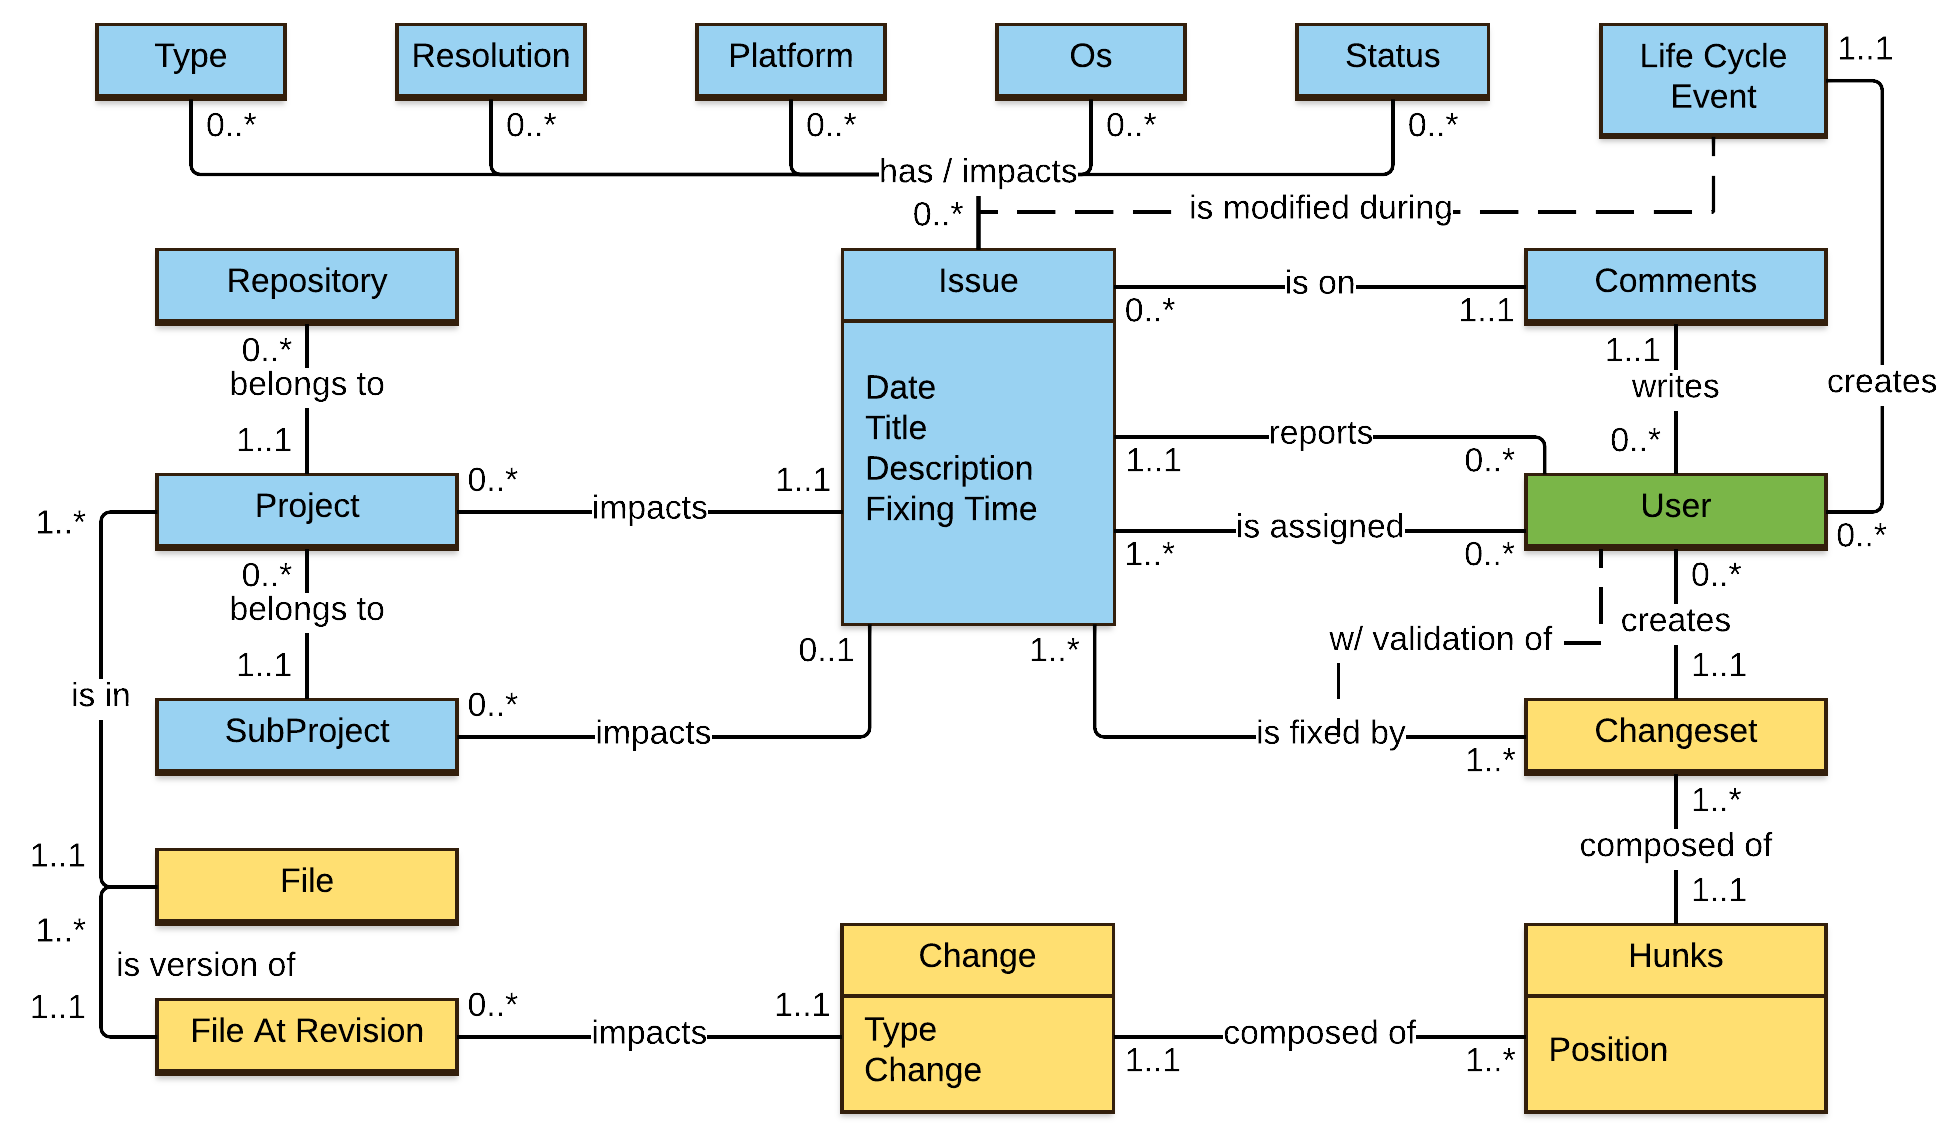
\includegraphics[width=0.8\textwidth]{media/Bumper-Model.png}
  \caption{BUMPER Metamodel\label{fig:bumper-metamodel}}
\end{figure*}

The BUMPER data model contains information found
in many common bug reporting and source code versioning
systems. More particularly, BUMPER data model revolves
around three main entities (1) Bug reports, (2) Changesets,
and (3) Hunks. Bug reports can contain zero or many
changesets---some bug reports such as duplicates do not
require changesets. A changeset may contain one or many
hunks. We carefully examined a large set of tools to define
the characteristics of each entity so as to provide support
for various types of analyses.
A bug report is characterized by the following features:

\begin{itemize}

  \item \textbf{ID}: A unique identifier
  \item 	\textbf{Dataset}: The dataset where the bug is extracted from
  \item 	\textbf{Date}: The bug submission date
  \item 	\textbf{Title}: The title of the bug report
  \item 	\textbf{Description}: The description of the bug
  \item 	\textbf{Project}: The project affected by this bug
  \item 	\textbf{Sub\_project}: The sub-project that this bug affects.
  \item 	\textbf{Version}: the version of the project that this bug
  affects
  \item 	\textbf{Impacted\_platform}: The platform that this bug
  affects
  \item 	\textbf{Impacted\_OS}: The operating system that this bug
  affects
  \item 	\textbf{Bug\_status}: The status of the bug
  \item 	\textbf{Resolution}: A description on how the bug was
  resolved
  \item 	\textbf{Reporter\_pseudo}: The pseudonym of the person who
  report the bug
  \item 	\textbf{Reporter\_name}: The name of the person who
  reported the bug
  \item 	\textbf{Assigned\_to\_pseudo}: The pseudonym of the person
  who has been assigned to fix the bug
  \item 	\textbf{Assigned\_to\_name}: The name of the person who has
  been assigned to fix the bug
  \item 	\textbf{Bug\_severity}: The severity of the bug
  \item 	\textbf{Fixing\_time}: The time in minutes it took to fix the
  bug
  \item 	\textbf{Comment\_nb}: The number of comments posted on
  the bug report system for that bug
  \item 	\textbf{Comment}: The comments associated with the bug.
  \item 	\textbf{File}: The name of the source code file that have been
  modified to fix a bug.
\end{itemize}


A changeset is represented using the following features:

\begin{itemize}

  \item 	\textbf{ID}: The unique identifier, represented as an SHA-1
  hash
  \item 	\textbf{User}: The name and email of the person who
  submitted the commit
  \item 	\textbf{Date}: The date at which this commit has been fixed
  \item 	\textbf{Summary}: The commit message entered by the user
  \item 	\textbf{File}: The fully qualified name of a file modified on
  that commit. A changeset can have one or many files.
  \item 	\textbf{Number\_files}: The number of files that have been
  modified in that commit
  \item 	\textbf{Insertions}: The number of inserted lines
  \item 	\textbf{Deletions}: The number of deleted lines
  \item 	\textbf{Churns}: The number of modified lines
  \item 	\textbf{Hunks}: The number of consecutive lines that have
  been changed
  \item 	\textbf{Parent\_bug}: The id of the bug this changeset belongs
  to.
\end{itemize}


\section{How to use this dataset}

In this section, we present how developers and researchers have and could use our dataset.

\subsection{Finding bug-fix}
\label{subs:Bug Fixing}

BUMPER\cite{Nayrolles2015d,Nayrolles2016}\footnote{https://bumper-app.com}, is a search engine for bug-fix in same way as Google is a search engine for websites. BUMPER uses Apache Solr\cite{Nayrolles2014b} to provide natural language searches of bug report and fixes.
This can help developers, engineers and computer science students not only to find patch to a given bug but also discover how experienced open-source developers write fixes.

\subsection{Studying bug-fix relationships and patterns}
\label{subs:Studying bug-fix relationships}

We see our dataset as way to facilitating research in the area
of mining bug repositories and more particulary, bug-fix relationships and patterns\cite{Kim2013e,Saha2014,Martinez2014}. Studying software repositories to gain insights
into the quality of the code is a common practice.
However, this task requires
time and skills in order to download and link all the pieces of informations
needed for adequate mining. Moreover, our dataset is available in JSON\footnote{https://bumper-app.com/msr16.json}, CSV\footnote{https://bumper-app.com/msr16.csv} and XML\footnote{https://bumper-app.com/msr16.xml} so one can choose his favorite format to work with.

\subsection{Comparing Approaches}
\label{sub:Comparing Approaches}

In bug reproduction\cite{Chen2013,Nayrolles2015}, prediction\cite{Kamei2010,Bhattacharya2011}, triage\cite{Anvik2006,Jeong2009m,Kong2011} and other related fields of software maintenance and evolution, comparing approaches is often taxing as datasets might not be publicly avalaible of the way data are gathered can be unclear.
With our dataset, approches could be more easily compared to each other.

In short, our dataset that can be used by software practitioners
and researchers to analyse (efficiently) bugs and their fixes without having
to go from one repository to another, worry about the way data is represented
and saved, or create tools for parsing and retrieving various data attributes.
We hope that the community embraces this dataset and evolve it with even more bug and projects.

\section{Conclusion}
\label{sec:Conclusion}

In this paper, we presented a dataset that we built to offer developers and
researchers the ability to access various bug-related data
from diverse repositories in a single dataset. This paper
contributes also with a large dataset with 732,406 bugs,
1,645,252 changesets, 457,663 files that have been modified to fix the bugs
and 1,930 distinct project
related to Netbeans, the Apache Software foundation's
software, Eclipse and Gnome. The dataset is publicly available at https://bumper-app.com/msr16.

As future work, we want to improve our dataset by
adding more projects such as project hosted on Github and the Mozilla
Foundation datasets. Also, we intend to add other features
such as the number of times a bug is reopened, the number
of times a bug has been duplicated, etc.

%
% End generated code
%

%
%  Use this command to print the description
%


% The following two commands are all you need in the
% initial runs of your .tex file to
% produce the bibliography for the citations in your paper.
\bibliographystyle{abbrv}
\bibliography{library}  % sigproc.bib is the name of the Bibliography in this case
% You must have a proper ".bib" file
%  and remember to run:
% latex bibtex latex latex
% to resolve all references
%
\end{document}
